\documentclass[10pt,twocolumn,letterpaper]{article}

\usepackage{cvpr}
\usepackage{times}
\usepackage{epsfig}
\usepackage{graphicx}
\usepackage{amsmath}
\usepackage{amssymb}
\usepackage{subcaption}
\usepackage{booktabs}
\DeclareMathOperator*{\argmax}{arg\,max}
\DeclareMathOperator*{\argmin}{arg\,min}

% Include other packages here, before hyperref.

% If you comment hyperref and then uncomment it, you should delete
% egpaper.aux before re-running latex.  (Or just hit 'q' on the first latex
% run, let it finish, and you should be clear).
\usepackage[breaklinks=true,bookmarks=false]{hyperref}

\cvprfinalcopy % *** Uncomment this line for the final submission

% \def\cvprPaperID{****} % *** Enter the CVPR Paper ID here
\def\httilde{\mbox{\tt\raisebox{-.5ex}{\symbol{126}}}}

% Pages are numbered in submission mode, and unnumbered in camera-ready
%\ifcvprfinal\pagestyle{empty}\fi
\setcounter{page}{1}
\begin{document}

%%%%%%%%% TITLE
\title{Generating Audio for Muted Piano-Playing Video using Deep Learning}

\author{XIA Junzhe\\
{\tt\small 20493411}\\
{\tt\small jxiaaf@connect.ust.hk}
\and
YANG Baichen\\
{\tt\small 20493198}\\
{\tt\small byangak@connect.ust.hk}
\and
HUANG Zeyu\\
{\tt\small 20493631}\\
{\tt\small zhuangbi@connect.ust.hk}
}

\maketitle

% Todo: Determine whether we need to introduce notation at introduction
%

%%%%%%%%% ABSTRACT
\begin{abstract}
   It is noticed that human playing the piano effectively generates a series of well-patterned actions, i.e. the position of hands and the keys and the depth of keys being pressed down. 
   The notes that the piano generates strongly obey to this visual pattern. 
   Hence, it becomes reasonable to recognize the visual patterns from piano-playing videos and reproduce the instrumental sounds using machine learning.
   In this project, we are going to propose a deep learning approach to effectively recognize key-press gestures and produce corresponding audios afterwards.
   
\end{abstract}

%%%%%%%%% BODY TEXT
\section{Introduction}
\label{Introduction}
   The production and consumption of digital music and video are thriving in recent years, and related researches in music and video recognition have become rather important in related fields.
   Among these fields, one important problem is how to construct mapping from videos to songs, which is possible because the visual representation is a vital aspect of musics.
   To be more specific, how to conduct the conversion from video information to symbolic notation such as music scores or Musical Instrument Digital Interface (MIDI) file.
   This problem is quite realistic for music lovers as it is hard to replay a music video without music transcription support.
   
   Our target is to generate music transcription and corresponding audio from piano-playing videos without any sound information.
   Previous works have been done towards this problem by implementing traditional computer vision methods for this task.
   However, evaluation results show that these methods are either not accurate or easy to be influenced by environmental conditions.
   So in this report, we propose a more robust solution for piano video recognition and music re-generation.

   To specify the problem, we introduce the following notations:

   Given a muted piano playing video $\vec{V}$ where the whole keyboard should be in the screen and each key can be seen clearly.
   Our task is to figure out the black note set $T_i^B$ and the white note set $T_i^W$ which are played at specific frame $F_i$ extracted from $\vec{V}$ and concatenate the notes together to regenerate the piano sound for this video.
   The note set $T$ should contain the key-pressed information as well as velocity information.
   
   To accomplish this task, we divide it into three stages.

   \textbf{1) Keyboard Extraction}
   As the keyboard's location differs in different videos, the first step is to develop a method extracting the whole keyboard from the background and conduct rectification on it. 
   The extracted keyboard will be fed into the second step.

   \textbf{2) Keypress Recognition}
   After the keyboard area is extracted, our core task is to recognize finger-key correspondence and determine whether the keys are pressed or not. 
   To finish this recognition, we need to focus on the piano keys' arrangement pattern as well as the illumination circumstance.
   However, since there are often reflections, shadows and other visual noises cast on the keyboard, it is rather difficult to develop an algorithm based on traditional computer vision method.
   Therefore, a robust algorithm is required.

   \textbf{3) Velocity Evaluation}
   The velocity information is essential in audio emotion expression. 
   With a high velocity value, the song conveys stronger feelings, and vice versa. 
   Since the velocity is a kind of dynamic information, our algorithm need to analyze several neighbor frames simutaneously in order to get the estimation.

   We have developed methods to solve these three parts and received a quite good result. 
   For the \textit{Task 1}, we've tried both traditional computer vision methods and deep learning methods, finally determined to use the \textit{SIFT} method \cite{SIFT} to achieve a better outcome.
   About the \textit{Task 2}, we trained two different neural network models for black and white key-press detection. 
   Both neural network models adopt VGG-like structure\cite{VGG} with two or three layers structure as the key size is rather small for deeper convolutional neural network to learn.
   And lastly for the \textit{Task 3}, we use the LSTM structure \cite{LSTM} and feed in neighbor frames of a video to perceive the change of the keypress as well as the velocity.

   Currently, our recognition result is quite acceptable. For the keypress recognition accuracy, i.e. the music score generation, is about \(75\%\), which is notably better than traditional computer vision methods with accuracy around \(50\%\).
   And about the velocity detection, there is also a satisfactory result as the listeners can sense some emotion which is similar as the original song conveys.
   Furthermore, to get higher robustness, we've record our own dataset in addition to adopted dataset from previous researches in order to increase diversity of environmental conditions. 
   
%------------------------------------------------------------------------
\section{Related Work}
   Previous works have been done in related area and some of them are targeting at this specific problem. In this section we will give brief introduction for them and discuss their strengths and drawbacks.

   One previous solution was proposed in Gorodnichy and Yogeswaran's paper \cite{gorodnichy2006detection} where traditional computer vision method is utilized to complete the keyboard and hand extraction as well as the gesture recognition tasks.
   Detaily, this solution divides the problem into three parts: Keyboard image detection, Hand detection and Finger detection. 
   It compute the keyboard boundary according to the assumption that white keys are surrounded by nonwhite areas, i.e. the division algorithm is based on the contrast information.
   And for the hand and finger detection, it utilized the background subtraction method and crevice-detection method.
   This solution achieved this task only with traditional computer vision methods, whose cost is lower than neural network model as the latter one needs large dataset and training.
   However, these methods required a frame where there are no hands on the keyboard because the flood fill algorithm will fail if there is a hand involving in.
   Also, since illumination conditions may differ, this traditional computer vision method doesn't perform quite well under different circumstances.

   Another solution towards this problem was proposed by Akbari et al. \cite{Akbari} 
   They proposed a system of automatically annotating piano-playing video using convolutional neural networks (CNNs) and two separate binary support vector machines (SVMs).
   Though a high accuracy has been achieved in keyboard and hand detection, this solution tackles issues according to some artificially formulated rules related to the visual nature of the piano keyboard, which is hard to prove its correctness in most cases.
   Also, since it applies CNN method in all stages of the problem, the computational cost is rather high, which is unavoidable.

%------------------------------------------------------------------------
\section{Dataset}

   In this section, we will talk about our dataset source and pre-processing.

   We adopt our dataset mainly from two sources: \textbf{modified from the dataset that was been used in previous work done by Akbari \cite{Akbari}}; \textbf{our own record}.
   Both datasets are formed by two parts: muted piano-playing videos and corresponding MIDI file, where contains all the pitch and velocity information.

\subsection{Dataset Source}

   \subsubsection{Dataset from Previous Work}

   First part of our dataset is obtained from a previous research \cite{Akbari}. It consists of piano playing videos captured in different situations which may lead to enhancement of model's strength:

   \textbf{Camera Position} As variations in position may lead to keyboard detection failure, this dataset's recording position contains three posibilities: $+45,\ 0,\ -45$ degrees from vertial.

   \textbf{Pianists} This dataset includes $14$ different players with different hand sizes, playing styles and skin colors, which will increase robustness of the model.

   \textbf{Positive and Negative Examples} This dataset also include both positive and negative examples, where negative stands for moving the hands over the keyboard without pressing any key.\\
   
   \begin{minipage}{0.9\linewidth}
      \centering
   \begin{tabular}{ccc}
      \toprule
      \# of Frames&\# of Black&\# of White\\
      \midrule
      70540 & $\sim$600000 & $\sim$400000\\
      \bottomrule
      \end{tabular}
      \captionof{table}{Stats of Previous Dataset} \label{tab:prevdataset} 
   \end{minipage}
      
   \subsubsection{Our New Dataset}

   However, since the first part of our dataset doesn't include velocity information, we recorded our own dataset additionally to train the network.
   Despite of velocity information, our dataset also has the following several features:

   \textbf{High Resolution} Our dataset is recorded by $1080P$ camera. The keyboard resolution increased by $70\%$ than the previous dataset. We downsize the keyboard images into \(884 \times 106\) before feeding into the model, which is still even higher than the resolution of \cite{Akbari}'s dataset without downsizing.

   \textbf{Music} The first dataset only contains sequentially key-press sound track, which cannot represent real music piece. 
   In our dataset, we played and recorded several master pieces to simulate real piano-playing videos.\\

   \begin{minipage}{0.9\linewidth}
      \centering
   \begin{tabular}{ccc}
      \toprule
      \# of Frames&\# of Black&\# of White\\
      \midrule
      22266&14536&27843\\
      \bottomrule
      \end{tabular}
      \captionof{table}{Stats of Our Dataset} \label{tab:ourdataset} 
   \end{minipage}

\subsection{Dataset Preprocessing}

\subsubsection{Conversion from/to MIDI format}

To get a trainable dataset, we firstly align the beginnings and the ends of videos and MIDI audios and sample frames out of both media files in a sampling rate of $25$ fps. 
Then, we generates a \(N \times 88\) label for each video file recording the status of each piano key in each frame, where \(N\) stands for the number of frames in that video.

The output of our method is a matrix of similar shape. 
The matrix undergoes a reverse process to transform into a MIDI file with the same sampling rate.

\subsubsection{Single Key Separation}

After we get the standardized keyboard image \ref{keyboarddetection}, we need to further separate it into single white keys and single black keys for training.

As for white keys, we equally divide the width of the image into \(52\) parts in the sense that all white keys have the same width.
\[White_i = Image[0:Height, i \times \frac{Width}{52}: (i + 1)\times\frac{Width}{52}]\]

As for black keys, since different keyboard has different black keys layout. We extract the top \(5\) rows of the standardized keyboard image and use Otsu's Thresholding Algorithm to convert it into a binary image. Since most of cases, players' hands will not overlap with the very top part of the keyboard, we can expect that the image extracted has a black-white alternating pattern:

\begin{figure}[h!]
   \centering
   
\includegraphics[width=\linewidth, height=0.04\linewidth]{fig/17.jpg}
   \caption{Expected Extracted Image}
\end{figure}

Then we take the average value of pixels in each columns, then every white-to-black pixel has exactly the x-coordinate of a black key's left boundary, every black-to-white pixel has the x-coordinate of a black key's right boundary.

\[Left_i = \{x: avg_x > 0 \text{ and } avg_{x + 1} = 0\}_i\]
\[Right_i = \{x: avg_x = 0 \text{ and } avg_{x + 1} > 0\}_i\]

After we get the left and right boundary of each black key, we can localize every black key as following:
\[Black_i = Image[0:Height, Left_i : Right_i]\]

% In our implementation, we also set it possible to acquire arbitrary degree of forward/backward positive difference in case of need.

\section{Methods}

In this section we will talk about methods tried and their pros and cons. 
As discussed in Section \ref{Introduction}, we divide this problem into three stages, keyboard detection, keypress recognition and velocity evaluation.

\subsection{Keyboard Detection} \label{keyboarddetection}
\label{Keyboard}

Towards the keyboard detection problem, we've tried three methods. 

\subsubsection{Hough Line Detection}
Firstly, we adopted the traditional CV method Hough Line Detection into this task, which is shown in Figure \ref{fig:1}. 
% It first conduct Gaussian Blurring on the picture in order to avoid noise for edge detection. 
% Then the result will be fed into the Canny Edge Detector \cite{Canny}.
Firstly, we can obtain the edge information of the picture by conducting Gaussian Blurring and Canny Edge Detection on it.
Next, we apply Hough Line Transformation \cite{Hough} on the preprocessed picture to detect boundary lines candidates. 
And since there'll be several repeated boundary line detected, we prune those repeated lines according to their slopes and positions.
% , and from here we will get 3 to 5 boundary candidates.
Finally, we determine the exact two parallel lines that bound the keyboard by examining the black and white pixel location pattern. 
% That is, if we denote the distance between two boundary lines as $d$, then we select two lines to be boundary lines when the average pixel value in the upper \(\frac{2}{3}d\) is darker than that in the lower \(\frac{1}{3}d\).

\begin{figure}[h!]
      % \begin{subfigure}{0.23\textwidth}
      %   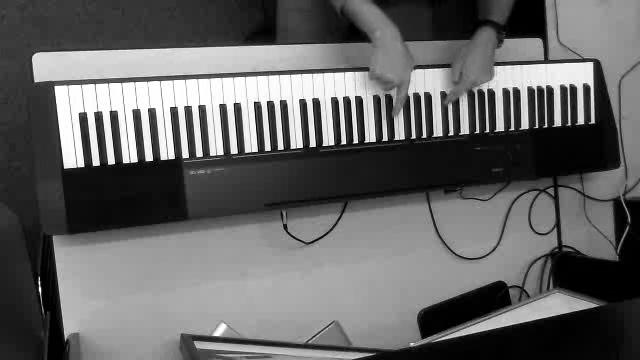
\includegraphics[width=\linewidth]{fig/1.jpg}
      %   \caption{Grayscaled Original Image} \label{fig:a}
      % \end{subfigure}\hspace*{\fill}
      \begin{subfigure}{0.23\textwidth}
        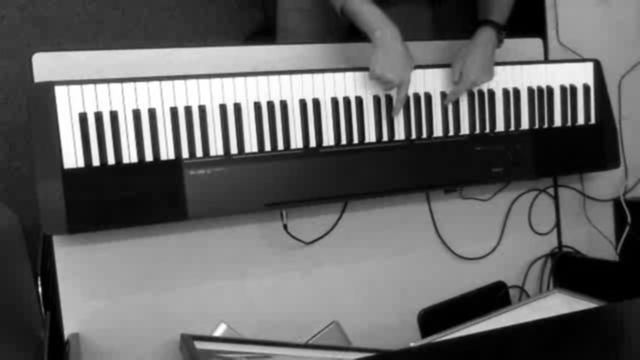
\includegraphics[width=\linewidth]{fig/3.jpg}
        \caption{Gaussian Blurred Image} \label{fig:b}
      \end{subfigure}\hspace*{\fill}
      % \medskip
      \begin{subfigure}{0.23\textwidth}
        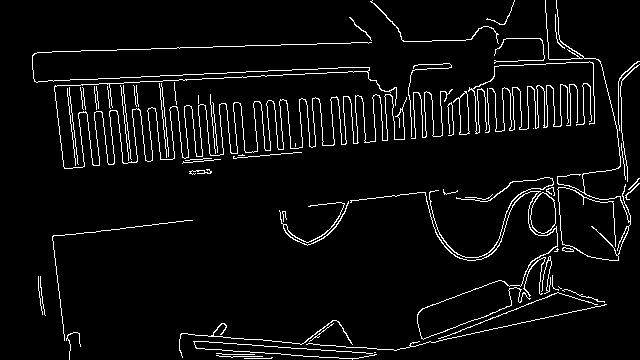
\includegraphics[width=\linewidth]{fig/4.jpg}
        \caption{Canny Edge Detection} \label{fig:c}
      \end{subfigure}
      \begin{subfigure}{0.23\textwidth}
        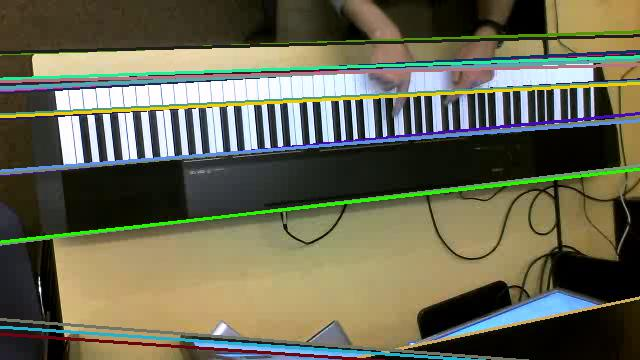
\includegraphics[width=\linewidth]{fig/5.jpg}
        \caption{Hough Line Transformation} \label{fig:d}
      \end{subfigure}\hspace*{\fill}
      % \medskip
      % \hspace{2.1cm}
      \begin{subfigure}{0.23\textwidth}
        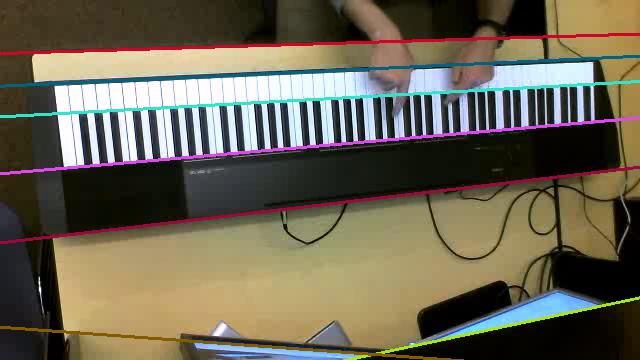
\includegraphics[width=\linewidth]{fig/6.jpg}
        \caption{Prune Repeated Lines} \label{fig:e}
      \end{subfigure}
      
      \caption{Hough Line Detection Method} \label{fig:1}
\end{figure}

However, this method has some major drawbacks. 
For one, the computational complexity of Hough Line Transformation is $O(n^3)$, where $n$ is the number of pixels. 
So the computation is quite expensive.
% Also, to achieve high accuracy, hyperparameters of Canny Edge Detector and Hough Line Transform varies a lot under different illumination circumstances.
% This leads to unstable detection performance.
In addition, to complete such detection, a frame without hand on the keyboard is needed, which is unobtainable for some videos.
Therefore, we resort to the second choice, using Deep Convolutional Neural Network.

\subsubsection{CNN Detection}

We next tried Convolutional Neural Network to detect the keyboard location. 
As the dataset doesn't offer us information about the exact location of keyboard, we manually labelled coordinates of the keyboard and feed them into a pre-trained ResNet-18 \cite{resnet} model for coordinate regression.

\begin{figure}[h!]
   \centering
   \begin{subfigure}{0.25\textwidth}
      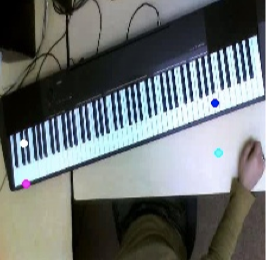
\includegraphics[width=\linewidth]{fig/8.png}
      \caption{Failure Example of CNN} \label{fig:f}
    \end{subfigure}
    \begin{subfigure}{0.30\textwidth}
      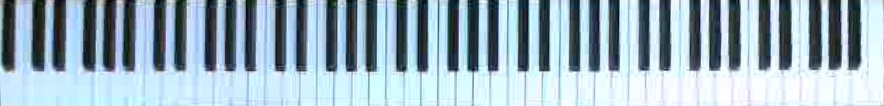
\includegraphics[width=\linewidth]{fig/9.jpg}
      \caption{SIFT Result} \label{fig:g}
    \end{subfigure}
   \caption{Comparison between CNN and SIFT} \label{fig:2}
\end{figure}

However, since the dataset is highly homogeneous because they are extracted from 71 videos, the model tends to build a mapping between image features to 71 fixed coordinate sets, which made the model’s performance on test set quite undesirable.
A failure example is shown in Figure \ref{fig:f}

We therefore turn to our third choice, the SIFT method.

\subsubsection{SIFT Detection}

Our finalized solution on this task is Scale Invariant Feature Transform (SIFT) \cite{SIFT}.

For each image in the dataset, we extract SIFT descriptors \(V_i^{1\times128}\) \((i=0,1,2,3)\) for pixel patches containing the four keyboard corners in each image using the coordinates we've labelled in the previous method.

In test time, we derive the four keyboard corners by finding the point whose SIFT descriptors are most similar to the ground truths, i.e.
$$P_i^* =\argmin_P\sum_{k=0}^{64}{\sqrt{\sum_{j=0}^{128}(V_j^P-V_{ij}^k)^2}}$$

The result shows that this method is quite robust and accurate in determining the keyboard location.
Under most circumstances, the method can extract the keyboard correctly and entirely.
A comparison example is shown in Figure \ref{fig:2}

\subsection{Keypress Recognition} \label{keypressdetection}

Now that we have obtained the extracted keyboard image from background, we are able to further conduct keypress recognition task on it. We will develop CNN models to accomplish this task.

\subsubsection{Loss Function}
The loss function we used is \textbf{Binary Cross Entropy Loss}, which can be described as following:
\begin{align*}
   w^*=&\argmin_w-\sum[y_i\log{w(x_i,\theta)} \\
      &+(1-y_i)\log(1-\log{w(x_i,\theta)})]+\lambda||w||_2
\end{align*}

The reason is that we are targeting at a binary labelling problem.
That is, our dataset $D = \{(x_1, y_1), (x_2, y_2), \cdots, (x_n, y_n)\}$ where $x_n\in\mathbb{R}^{C\times H\times W}$ is the images and $y_n\in\{0,1\}$ is the predicted probability of begin pressed, and data pairs are independent of each other.
After defining our loss function, our next step is to process the data and set up the network model.

\subsubsection{Whole Keyboard Detection}
\label{Keypress-keyboard}

   Our first attempt is to put the whole keyboard and corresponding frame note label into the neural network, trying to recognize both the pressing pattern as well as key location by one network.
   We utilized a deep convolutional neural network solution for this task since it could preserve spatial information of the picture and focus its attention on some particular region.
   The set our CNN structure is VGG-like, and the design is shown in the Figure \ref{fig:h}.

   This method doesn't require any further data processing on the data derived from Task \ref{Keyboard}.
   However, we failed to obtain a good result with this approach. 
   One major problem may be that in our training set, some keys are frequently pressed while some are rarely pressed.
   This inbalance of frequency could provide the model with wrong attention.
   Also, as hands are small compared to the whole keyboard, the network tends to focus on other factors such as illumination conditions instead of hand motions, which may lower the accuracy.

   \begin{figure}[h!]
      \centering
      \begin{subfigure}{0.4\textwidth}
         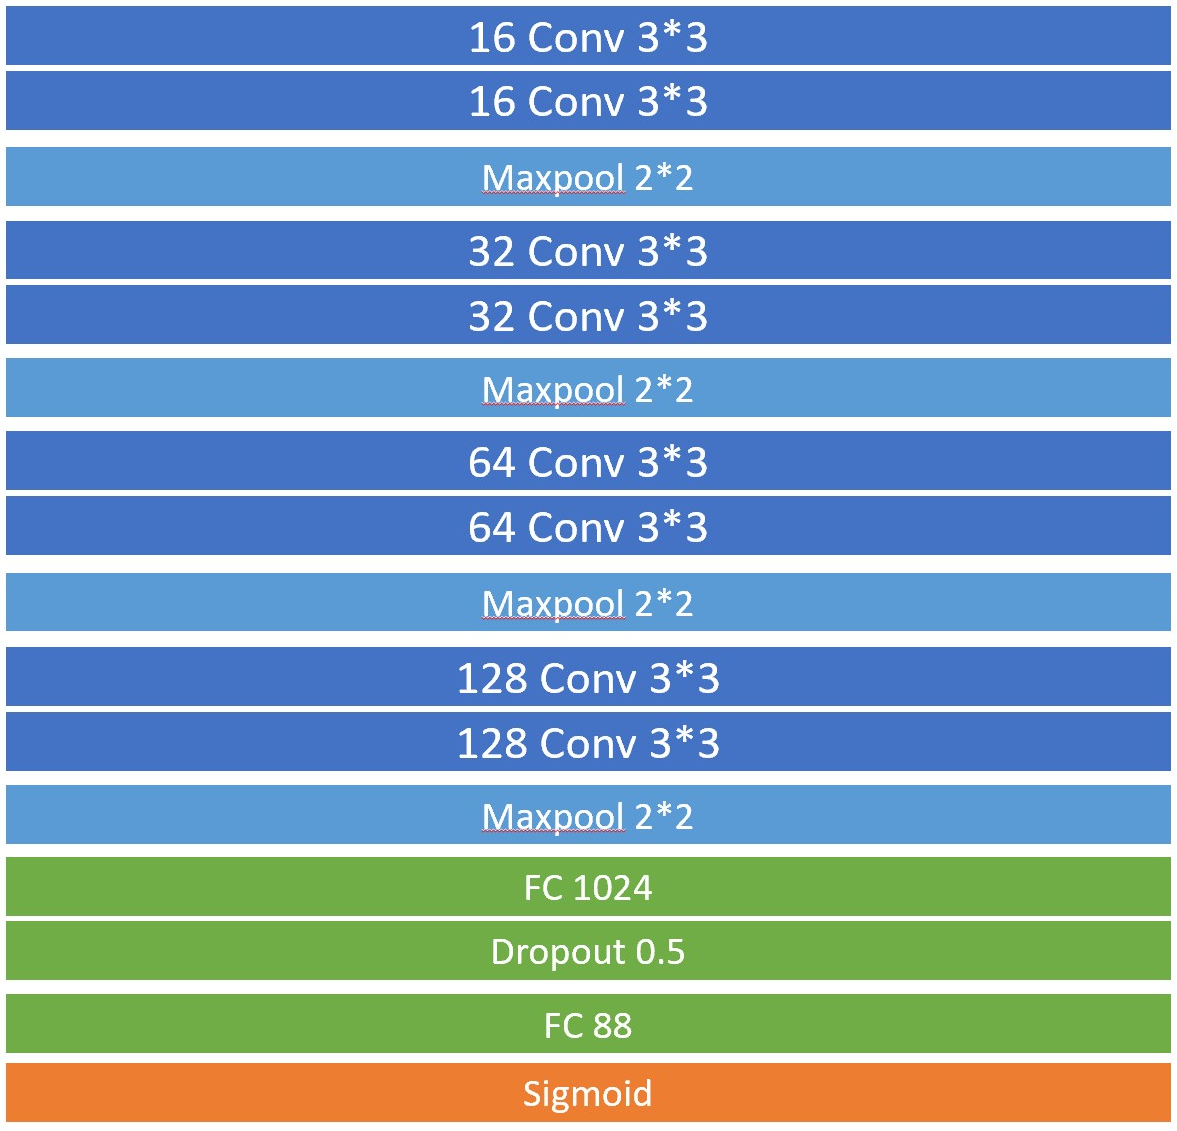
\includegraphics[width=\linewidth]{fig/10.png}
         \caption{CNN for Whole Keyboard Detection} \label{fig:h}
       \end{subfigure}
       \begin{subfigure}{0.4\textwidth}
         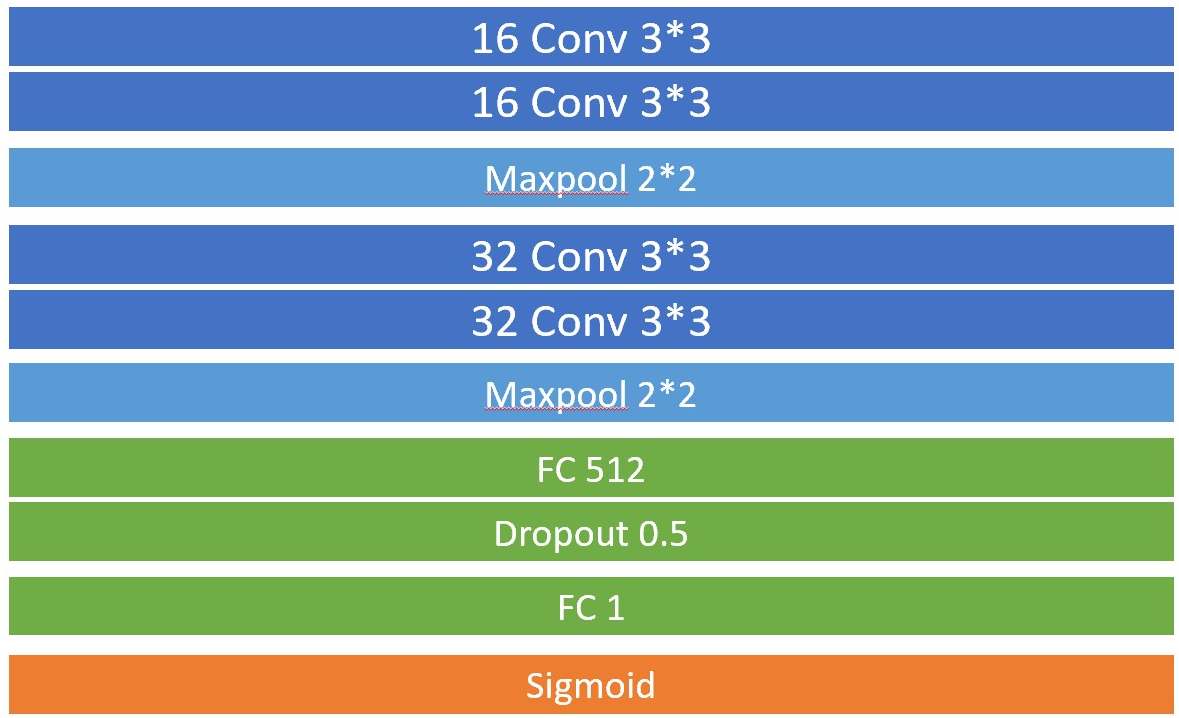
\includegraphics[width=\linewidth]{fig/11.png}
         \caption{CNN for Key Splitting} \label{fig:i}
       \end{subfigure}
       \begin{subfigure}{0.4\textwidth}
         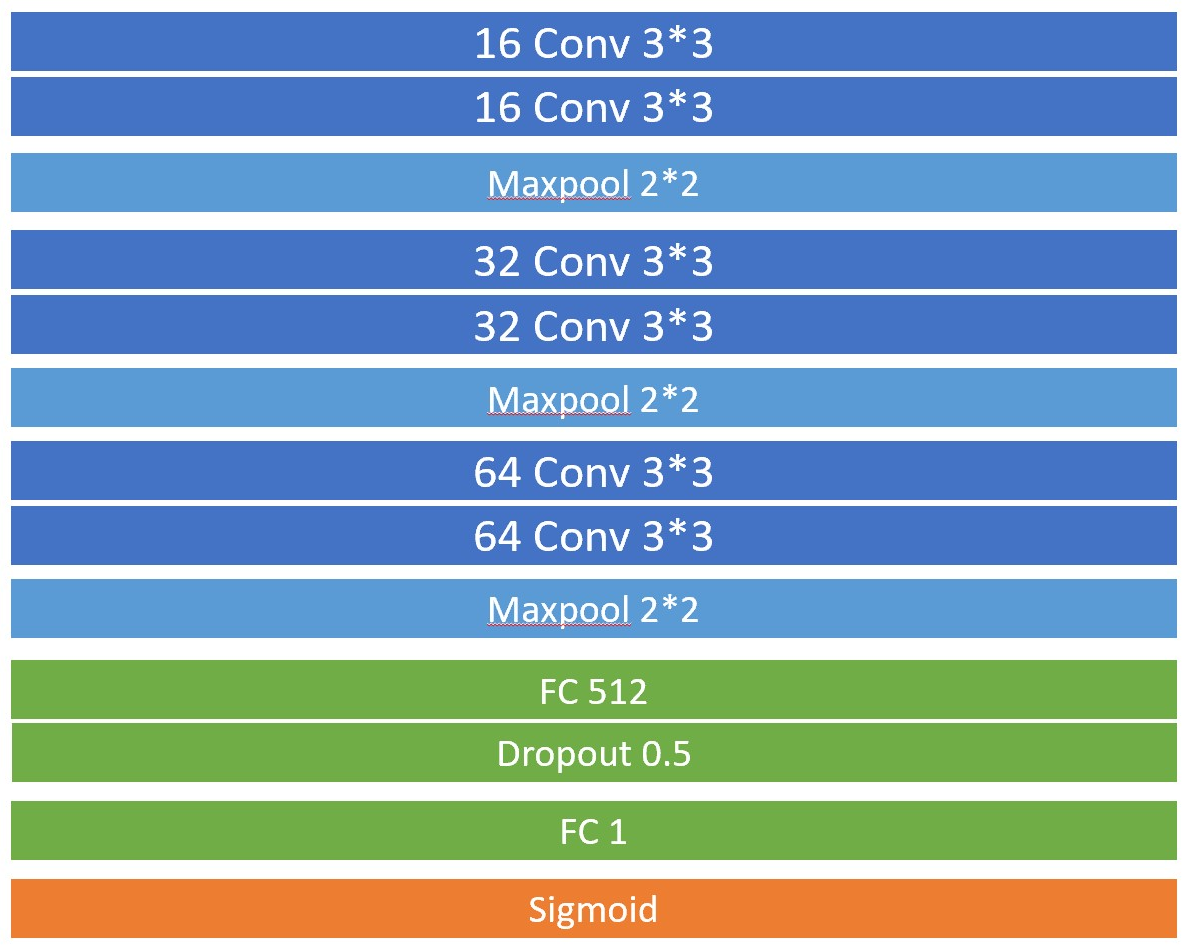
\includegraphics[width=\linewidth]{fig/12.png}
         \caption{CNN for Key Bundling} \label{fig:j}
       \end{subfigure}
      \caption{CNN structures for Keypress Recognition} \label{fig:3}
   \end{figure}

\subsubsection{Single Key Splitting}

To help direct the model's attention, in our next attempt we split the input image into 88 segments, 
each containing one piano key object at the center as our training target. 
Each white key is located by dividing a image into 52 pieces along the x-axis. 
Each black key is located using traditional cv algorithms. 
Since we have resized and skewed the images into standard \(884 \times 106\) rectangles, the splitting process yields a rather promising result. 
Finally, we add some ``tolerance'' by widening the cropped area by 2-4 pixels on its left and right sides to avoid the cropping area being to tight. 

We have trained two models for black and white keys respectively, each of the same structure shown in \ref{fig:i}.

This model works quite well on our dataset, and achieves higher accuracy than the previous method as we manually help direct the model's attention and eliminate the aforementioned frequency inbalance issue.

\subsubsection{Key Bundling}

\begin{figure}[h!]
   \begin{subfigure}{0.2\textwidth}
      \centering
      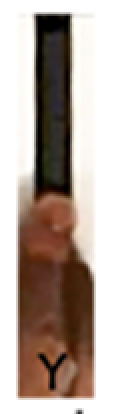
\includegraphics[width=0.26\linewidth]{fig/15.png}
      \caption{Single Key Split} \label{fig:k}
    \end{subfigure}\hspace*{\fill}
    \begin{subfigure}{0.2\textwidth}
      \centering
      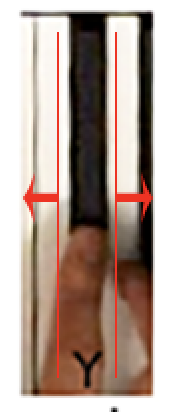
\includegraphics[width=0.4\linewidth]{fig/14.png}
      \caption{Key Bundling} \label{fig:l}
    \end{subfigure}
   \caption{Comparison between two splitting modes} \label{fig:4}
\end{figure}   

Lastly, we also introduce a second splitting stretegy called ``bundling'', where in this mode the ``tolerance'' is enlarged to include some neighbor keys.
In other words, we will produce images of several keys when the centered key is our training target. 

In our implementation, we make the number of neighbor keys to be bundled a variable hyperparameter. 
Since bundling too many keys tends to incur more noise, after some experiments we determined the bundling number to be $B = 3$, including exact one key on both sides. (See Figure \ref{fig:4})

The model we use to train bundled key images are shown in Figure \ref{fig:j}. 

Compared to the second method, it includes extra information about neighbor keys and hand motions without introducing the aforementioned inbalance problem either. However, more interference is introduced as well.

In our experiments, this approach outperforms the single key splitting approach in training set and validation set, but slightly weaker in the test set.

\subsection{Velocity Evaluation}

   Last part of our task is to evaluate the velocity of each keypress. 
   In MIDI file, the velocity is recorded as an integer value ranges from $0$ to $127$. 
   So our objective is to detect motion in ``pressed'' frames and neighbor frames and make a prediction on the velocity value of that key press.
   
   Since this prediction involves extracting features in a sequence, we use LSTM to tackle this problem. 
   
   \subsubsection{LSTM Architecture}

   In the sense of that velocity is related to how fast the keypress depth changes, which is also an important feature to determine whether a key is pressed, we used a CNN model pretrained in keypress detection \ref{keypressdetection} as the feature extractor for each input image. Then a sequence of feature tensors will be fed into a two-layer LSTM network with hidden size of 256, generating a single logit value.
   
   \[Velocity = Sigmoid(logit) * 127\]
   
After gating and rescaling this value, we will derive the final predicted velocity ranging from \([0, 128)\).

   \begin{figure}[h!]
      \centering
      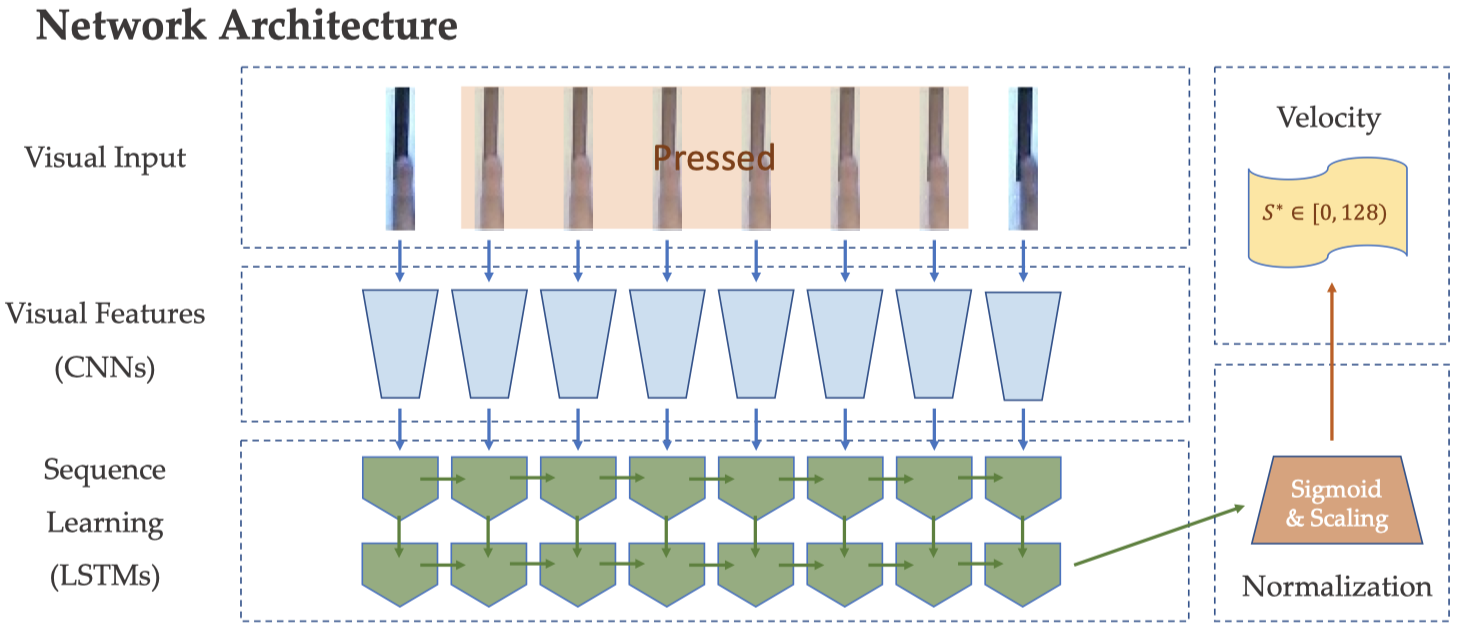
\includegraphics[width=\linewidth]{fig/13.png}
      \caption{LSTM Architecture for Velocity Evaluation} \label{fig:5}
   \end{figure}

   \subsubsection{Loss Function}

   The loss function we used is \textbf{Mean-Squared Loss} which can be described as following:

   \[w^*=\argmin_w[y - w(x, \theta)]^2+\lambda||w||_2\]

   While training, we used \(\text{sigmoid}\ (logit)\) as the final output of the network instead of \(\text{sigmoid}\ (logit) \times 127\).

\section{Experiments}

In this section we will talk about our experiment settings including the hyperparameters, and our current results.

\subsection{Keypress Recognition}

The whole keyboard network is deprecated in an early stage of our experiments due to its shortcomings mentioned in \ref{Keypress-keyboard}. 
Hence, the following experiment details only concern the single key and bundled key approaches, and there are four models in total.

\subsubsection{Hyperparameter Tuning}

All four models are trained \(200\) epoches with Adam optimizer with learning rate \(1e-3\), \(\beta_1 = 0.9, \beta_2 = 0.999, \epsilon = 1e-8\), and a learning rate decay by a multiplier of \(\gamma=0.05\) every $10$ epochs. 
We use a batch size of \(32\), and an \(L2\) penalty of \(0.1\) on the model parameters. 


\subsubsection{Evaluation Metrics}

To evaluate our keypress recognition performance, apart from the common accuracy, we also introduce two finer criterion: \textit{Precision} and \textit{Recall}.
\begin{align*}
   Precision &= \frac{TP}{TP+FP}\\
   Recall &= \frac{TP}{TP+FN}
\end{align*}
where
\begin{align*}
   TP &= \text{\# pressed keys predicted as ``pressed'' (True Positive)}\\
   FP &= \text{\# unpressed keys predicted as ``pressed'' (False Positive)}\\
   FN &= \text{\# pressed keys predicted as ``unpressed'' (False Negative)}
\end{align*}

We expect both metrics to be high. However, an increase in one often indicates a decrease in the other.
Thus, we introduce another commonly used metric named \textit{F1-Score}:
$$F1 = 2\cdot\dfrac{Precision\cdot Recall}{Precision + Recall}$$
to describe the recognition performance.

\subsubsection{Misleading Training Result}

In the very early stage, we use the raw dataset to feed the model during training and get following result:

\begin{minipage}{0.9\linewidth}
   \centering
\begin{tabular}{ccc}
   \toprule
   Precision &Recall&Accuracy\\
   \midrule
   1.39 \%& 2.04 \%&98.5\%\\
   \bottomrule
   \end{tabular}
   \captionof{table}{Misleading Training Result} \label{tab:prevdataset}

\end{minipage}

This result somehow revealed a very serious problem: most of the samples in the dataset are unpressed key images. So the model only need to output ``unpressed'', then a low loss and a high accuracy can be achieved. However, such a model is useless at all. Therefore, we need to perform some preprocess on dataset to make the training process meaningful.

\subsubsection{Reduce Dataset Unbalance}

To solve this dataset unbalance problem, we randomly took out some of the negative samples because most unpressed key images are almost the same, which are solely empty keys with no hand on it. Also, we upsampled those positive samples by simply duplicating them.

After applying this trick, the dataset contains almost the same number of positive samples and negative samples. We conducted some experiments with this improved dataset and concluded that this preprocess step prevented the model from only outputing only one result.

\subsubsection{Results}

We have reached \(90\%+\) training and validation accuracy on both black keys and white keys after applying the preprocessing mentioned above. 

Both Single and Bundle case splitting achieves quite good results.
The testset results are listed below:

\begin{minipage}{0.9\linewidth}
   \centering
\begin{tabular}{ccccc}
   \toprule
   & Precision &Recall&Accuracy& F1 Score\\
   \midrule
   \textbf{Bundle-B} &87.2 \%& 84.5 \%&99.9\%& 85.8\%\\
   \textbf{Bundle-W} &78.4 \%& 78.8 \%&98.2\%& 78.6\%\\
   \textbf{Single-B} &88.8 \%& 84.2 \%&99.9\%& 86.4\%\\
   \textbf{Single-W} &76.3 \%& 77.4 \%&98.1\%& 76.8\%\\
   \bottomrule
   \end{tabular}
   \captionof{table}{Final Result} \label{tab:prevdataset}

\end{minipage}

\subsection{Velocity Evaluation}

As for the LSTM network for velocity evaluation, we adopted pretrained CNN models for single white keypress and single black keypress as feature extractors. While training, we froze CNN networks to mainly improve the performance of the LSTM model.

\subsubsection{Hyperparameter Tuning}

Black key model are trained \(500\) epoches with Adam optimizer with learning rate \(5e-3\), \(\beta_1 = 0.9, \beta_2 = 0.999, \epsilon = 1e-8\), and a multiplier decay of \(\gamma=0.05\) for every $100$ epochs. We use a batch size of \(1\), and an \(L2\) penalty of \(0.005\) on the model parameters.

White key model are trained \(450\) epoches with Adam optimizer with learning rate \(5e-3\), \(\beta_1 = 0.9, \beta_2 = 0.999, \epsilon = 1e-8\), and a multiplier decay of \(\gamma=0.05\) for every $90$ epochs. We use a batch size of \(1\), and an \(L2\) penalty of \(0.005\) on the model parameters. 

\subsubsection{Evaluation Metrics}

To evaluate the velocity evaluation performance, we use average L1 Loss to measure the predicted velocity values and ground truths.

\[Average\ L1\ Loss = \frac{1}{N}\sum_{i=1}^{N}|\widehat{y_i} - y_i|\]

\subsubsection{Results}

In the model for white key velocity evaluation, we reached an average L1 Loss of \(12.4729\) on test set with the best model. In the model for black key, an average L1 Loss of \(12.2698\) is reached on test set with the best model.

\begin{figure}[h!]
   \begin{subfigure}{0.5\textwidth}
      \centering
      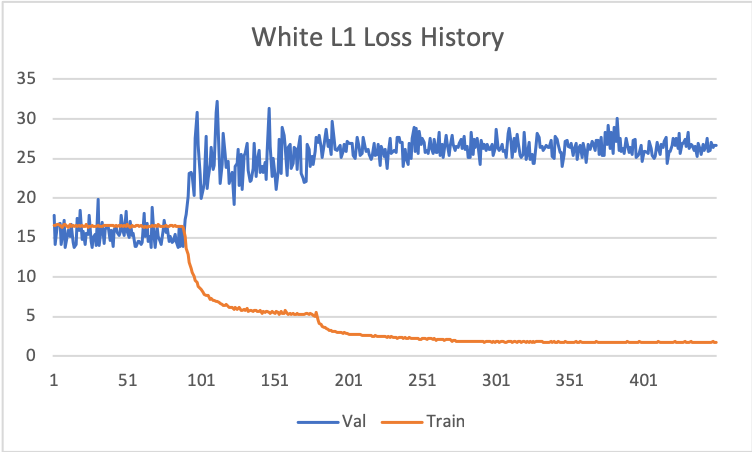
\includegraphics[width=\linewidth]{fig/vel_1.png}
      \caption{White L1 Loss History} \label{fig:k}
    \end{subfigure}\hspace*{\fill}
    \newline \newline
    \begin{subfigure}{0.5\textwidth}
      \centering
      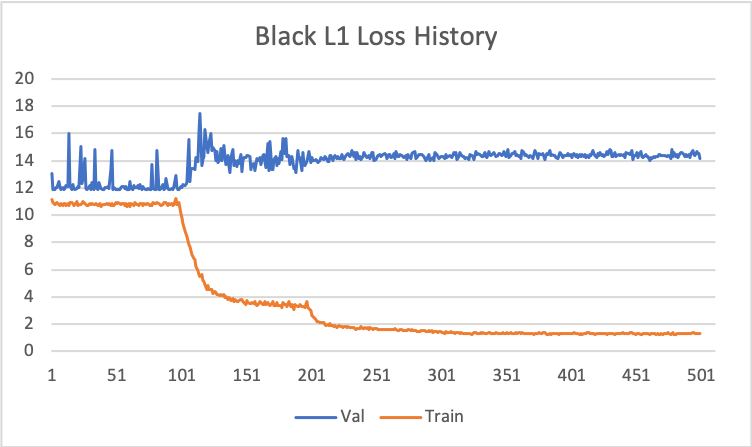
\includegraphics[width=\linewidth]{fig/vel_3.png}
      \caption{Black L1 Loss History} \label{fig:k}
    \end{subfigure}\hspace*{\fill}
   \caption{Stats during Training Process} \label{fig:6}
\end{figure}   

However, we believe there still exists large gap between our models and ideal models for velocity evaluation. Because considering the velocity only ranges from \(0\) to \(127\), a L1 loss of around \(12\) is far from a neglectable difference.

According to the loss history diagrams, we may need to cope with overfit problem emerged after the first \(100\) epoches. We have tried adding dropout on LSTM and CNN, as well as enlarging the regularization term in loss, but no satisfactory results have been obtained.

Demo Video

\section{Conclusion and Future Work}

In this paper, we've introduced a method to tackle the audio generation problem and achieves quite good performance.
Through our method, we could get the music score from a muted piano-playing video with a high accuracy.
And by this music score as well as the velocity information predicted, we are able to re-generate the audio with emotion.
Comparing to previous solutions, our method achieves either better accuracy or becomes more robust under different circumstances.

In the future, we plan to refine our velocity evaluation structure to achieve a better and more stable prediction result.
Also, we hope to implement a real-time recognition system to realize immediate pitch detection.


{\small
\bibliographystyle{ieee}
\bibliography{egbib}
}

\end{document}
